%%
%% The official i6 slide template _demo_
%% created by Philippe Dreuw and Thomas Deselaers, 2005
%%
%% $Id: slides.tex,v 1.48 2007-11-14 17:13:01 dreuw Exp $
%%
%% Possible options for:
%%  - language       : 'english' (default), 'german'
%%  - page numbering : 'nonumber', 'lastpage' to enable automatic page n/m numbering, 
%%                     'userlastpage' to enable a user defined page n/m numbering using \LastPage command,  
%%                      or leave empty for normal page numbering (default)
%%  - itemize        : 'triangle' or leave empty for bullets (default)
%%  - page titles    : 'allowpagebreaks' to enable titles with automatic page breaks, 
%%                     'nopagebreaks' to disable (default)
%%  - page layout    : 'vertical' to enable vertical centering on each slide using \vfill ... \vfill (default)
%%  - encoding       : 'utf-8' to enable utf encoding instead of latin1 (default)
%%  - tools          : 'blackslide' to insert a black slide which is linked with every slide title, e.g. to write a proof on the blackboard
%%
\documentclass[11pt, a4paper, landscape]{article}
\usepackage{NeyDreuwSlides_Nov07}


%%%%%%%%%%%%%%%%%%%%%%%%%%%%%%%%%%%%%%%%%%%%%%%%%%%%%%%%%%%%%%%%%%%%%%%%%%%%%%%%
%% flyspell can read the local ispelldict variable to automatically change the dictionary, 
%% e.g. german-new8, american, english, british, ...
%% 
%% Local IspellDict: american
%% 


%%%%%%%%%%%%%%%%%%%%%%%%%%%%%%%%%%%%%%%%%%%%%%%%%%%%%%%%%%%%%%%%%%%%%%%%%%%%%%%%
% custom packages
\usepackage{fancyvrb} %%% fancy verbatim to enable coloring within verbatim environments

%\usepackage{pst-node} 

%%%%%%%%%%%%%%%%%%%%%%%%%%%%%%%%%%%%%%%%%%%%%%%%%%%%%%%%%%%%%%%%%%%%%%%%%%%%%%%%
% Some example hacks work only in combination with the 'pdflatex -shell-escape'
% mode. Try 'make hacks'


%%%%%%%%%%%%%%%%%%%%%%%%%%%%%%%%%%%%%%%%%%%%%%%%%%%%%%%%%%%%%%%%%%%%%%%%%%%%%%%%
\renewcommand*{\title}{Graph-Based Image Segmentation}        % main title of the work (used for \TitlePage)
\renewcommand*{\titleshort}{Graph-Based Segmentation}         % short title (used for \lfoot)
\renewcommand*{\occasion}{Seminar Medical Image Processing -- MedBV13}		% (used for \TitlePage)
\renewcommand*{\occasionshort}{MedBV13}               % short occasion title (used for \rfoot)
%\renewcommand*{\date}{11. April 2005}                                        % default is \today (used for \TitlePage and \rfoot)
\renewcommand*{\author}{Phan-Anh Nguyen, Christian Oberdoefer}         % all the authors of the work, can be long (used for \TitlePage)
\renewcommand*{\authorshort}{Phan-Anh et al.:\xspace}                            % all the authors of the work, should be short (used for \lfoot)
\renewcommand*{\email}{\url{anh.nguyen@rwth-aachen.de, oberdoefer@i6.informatik.rwth-aachen.de}}  % all email address(es) of the authors (used for \TitlePage)
\renewcommand*{\mainauthor}{Phan-Anh Nguyen}                                   % the author(s) who presented the work (used for \TitlePage)
\renewcommand*{\mainauthoremail}{\url{anh.nguyen@rwth-aachen.de}}    % presenter mail address(es) (used for \FinalPage)
\renewcommand*{\www}{http://www-i6.informatik.rwth-aachen.de/}                % web address (used for \TitlePage _and_ \FinalPage)
\newcommand*{\keywords}{Graph Cut, Segmentation}                               % keywords, can be used for PDF summary

% will be set into the PDF document summary
\hypersetup{
  pdftitle={\title}, 
  pdfsubject={\occasion},  
  pdfauthor={\author}, 
  pdfkeywords={\keywords},
  % enable automatic page transitions: for endless loop edit in
  % acrobat reader -> preferences -> full screen -> after every X
  % seconds and after last page
  pdfpageduration = 2, 
%  pdfpagetransition = {Glitter /Di 315 /D 5}  
  pdfpagetransition = {Box /M /O /D 1},
}

%%%%%%%%%%%%%%%%%%%%%%%%%%%%%%%%%%%%%%%%%%%%%%%%%%%%%%%%%%%%%%%%%%%%%%%%%%%%%%%%
\listfiles
%%%%%%%%%%%%%%%%%%%%%%%%%%%%%%%%%%%%%%%%%%%%%%%%%%%%%%%%%%%%%%%%%%%%%%%%%%%%%%%%
\begin{document}

%%%%%%%%%%%%%%%%%%%%%%%%%%%%%%%%%%%%%%%%%%%%%%%%%%%%%%%%%%%%%%%%%%%%%%%%%%%%%%%%
\TitlePage

%%%%%%%%%%%%%%%%%%%%%%%%%%%%%%%%%%%%%%%%%%%%%%%%%%%%%%%%%%%%%%%%%%%%%%%%%%%%%%%%
\NewPage\headline{Outline}
%\small
\vfill
\begin{enumerate}
\item \hyperlink{sli:introduction}{Introduction and Motivation}
\item \hyperlink{sli:features}{Image Features}
%\begin{itemize}
%	\item \hyperlink{sli:surf}{Speeded Up Robust Features}
%	\item \hyperlink{sli:gPb}{Globalized Probability of Boundary}
%\end{itemize}
\item \hyperlink{sli:supervised}{Segmentation with Supervised Training}
%\begin{itemize}
%	\item \hyperlink{sli:svm}{Support Vector Machine for Region Ranking}
%	\item \hyperlink{sli:logistic}{Logistic Regression}
%	\item \hyperlink{sli:ssm}{Statistical Shape Model}
%\end{itemize}
\item \hyperlink{sli:construction}{Graph Construction}
\begin{itemize}
	\item \hyperlink{sli:region_graph}{Region Graph}
	\item \hyperlink{sli:contour_graph}{Contour Graph}
	\item \hyperlink{sli:mrf}{Markov Random Field}
\end{itemize}
\item \hyperlink{sli:algorithms}{Graph Cut Algorithms}
%\begin{itemize}
%	\item \hyperlink{sli:PCST}{Prize-Collecting Steiner Tree}
%	\begin{itemize}
%		\item \hyperlink{sli:branch_and_cut}{Branch-and-Cut Algorithm}
%	\end{itemize}
%	\item \hyperlink{sli:contour_cut}{Contour Cut}
%	\begin{itemize}
%		\item \hyperlink{sli:circulation}{Graph Circulations}
%		\item \hyperlink{sli:cost}{The Cost Function}
%		\item \hyperlink{sli:solution}{Computational Solution}
%	\end{itemize}
%	\item \hyperlink{sli:graph_cut}{Graph-Cut}
%	\begin{itemize}
%		\item \hyperlink{sli:min_cut}{Min-Cut Algorithm}
%		\item \hyperlink{sli:multi_shape}{Multi-Shape Graph-Cuts}
%	\end{itemize}
%\end{itemize}
\item \hyperlink{sli:application}{Applications}
%\begin{itemize}
%	\item \hyperlink{sli:ERS}{Efficient Region Search for Object Detection}
%	\item \hyperlink{sli:contour_detector}{Salient Contour Detection}
%	\item \hyperlink{sli:lung_segmentation}{Multi-Shape Graph-Cut for Lung Segmentation}
%\end{itemize}
\item \hyperlink{sli:conclusion}{Conclusion}
\end{enumerate}
\vfill
%\centerline{\footnotesize PS: the outline should not have more than 5-7 items
%  without any subitems}
%\normalsize
%\vfill


%%%%%%%%%%%%%%%%%%%%%%%%%%%%%%%%%%%%%%%%%%%%%%%%%%%%%%%%%%%%%%%%%%%%%%%%%%%%%%%%
\NewPage\headline{Literature} 
\vfill 
\begin{itemize}
\item S. Vijayanarasimhan and K. Grauman. \alert{Efficient region search for object detection.} Computer Vision and Pattern Recognition (CVPR), 2011 IEEE Conference, pages 1401--1408, June 2011.
\item R. Kennedy, J. Gallier, and Jianbo Shi. \alert{Contour cut: Identifying salient contours in images
by solving a hermitian eigenvalue problem.} Computer Vision and Pattern Recognition (CVPR), 2011 IEEE Conference, pages 2065--2072, June 2011.
\item Nakagomi, K. and Shimizu, A. and Kobatake, H. and Yakami, M. and Fujimoto, K. and Togashi, K. \alert{Multi-shape graph-cuts and its application to lung segmentation from a chest CT volume.}
\end{itemize}
\vfill


%%%%%%%%%%%%%%%%%%%%%%%%%%%%%%%%%%%%%%%%%%%%%%%%%%%%%%%%%%%%%%%%%%%%%%%%%%%%%%%%
\NewPage\headline{Introduction and Motivation} 
\hypertarget{sli:introduction}
\vfill
\begin{itemize}
\item Purposes of segmentation
\begin{itemize}
	\item Computer-aided diagnoses
	\item Object detection and segmentation for autonomous systems
	\item Shape alignments
\end{itemize}
\item Current problems
\begin{itemize}
	\item deformable shapes
	\item time constraint
	\item no clear boundaries
\end{itemize}
\item Advantages of Graph Representation
%\begin{itemize}
%	\item Flexible expression of constraints 
%	\item Powerful graph algorithms exist\\
%	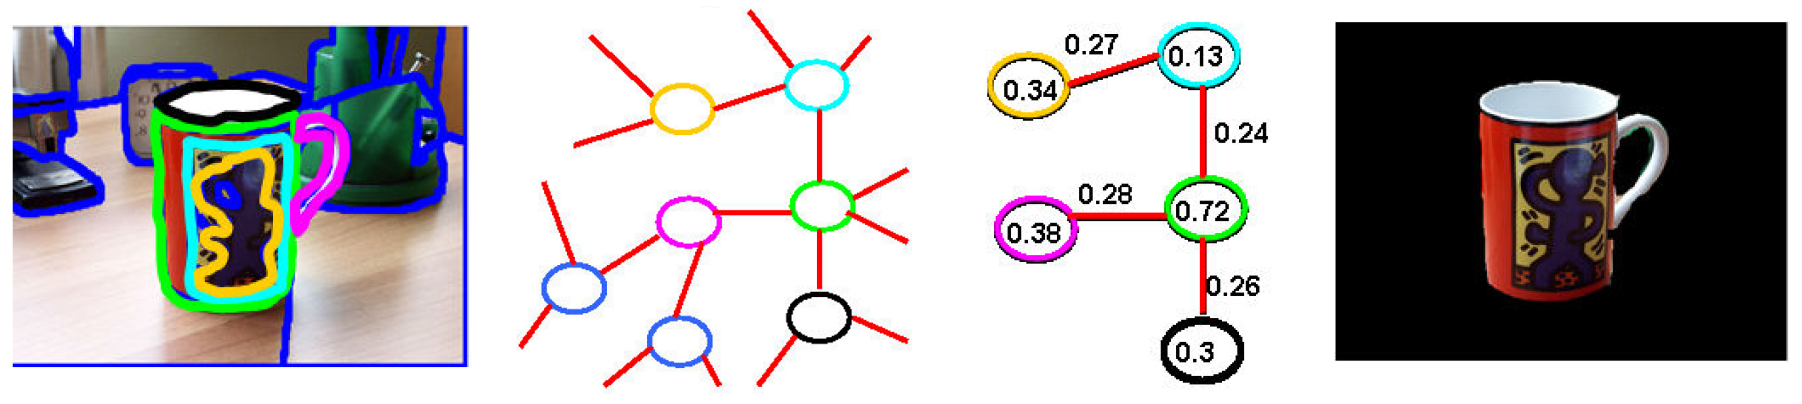
\includegraphics[width=.6\linewidth]{region_graph_intro}
%\end{itemize}
\begin{table}
  \centering
  \begin{tabular}{@{} M{.4\linewidth} M{.6\linewidth} @{}}
  	\begin{itemize}
  		\item Flexible expression of constraints 
  		\item Powerful graph algorithms exist
    \end{itemize}
      &
    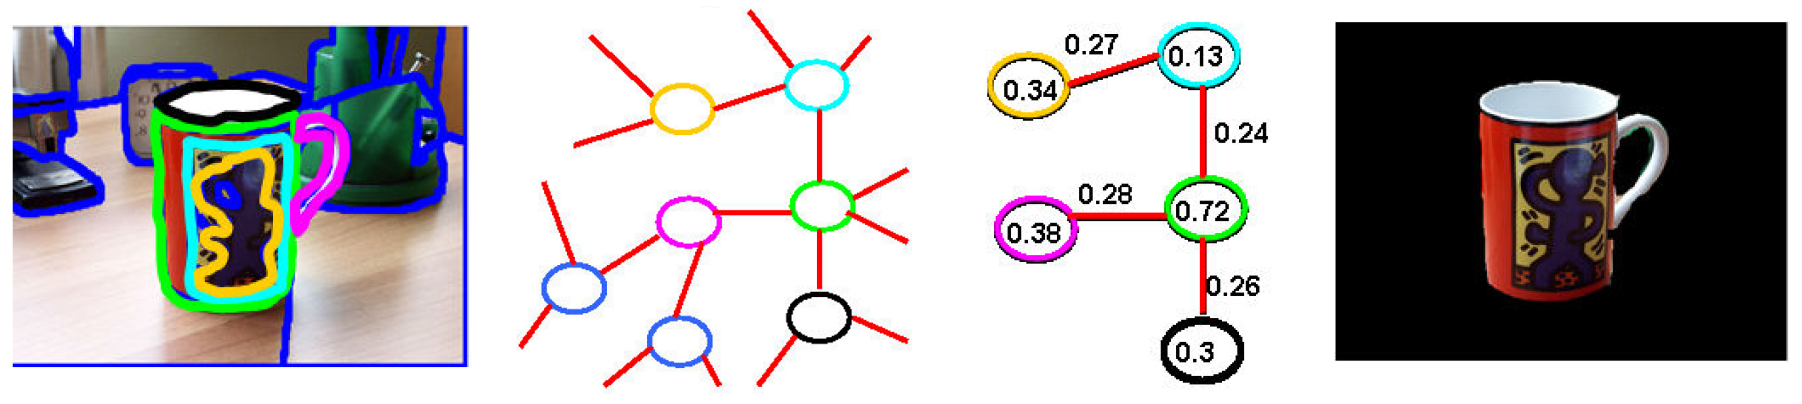
\includegraphics[width=.9\linewidth]{region_graph_intro}
  \end{tabular}
\end{table}

\end{itemize}
\vfill



%%%%%%%%%%%%%%%%%%%%%%%%%%%%%%%%%%%%%%%%%%%%%%%%%%%%%%%%%%%%%%%%%%%%%%%%%%%%%%%%
\NewPage\headline{Image Features: Speeded Up Robust Features}
\hypertarget{sli:style}
\vfill
\begin{itemize}
\item Detect interest points: $det(Hessian(I)) = I_{xx}I_{yy} - I^2_{xy}$
\item Orientation assignment (rotation invariant): select the dominant direction of Haar wavelet response vectors $(d_x, d_y)$.
\item SURF is computed within a window of size $20s$.
\item Further split the window into $4 \times 4$ sub-windows.
\item[]
  \begin{figure}
    \centering
    \begin{tabularx}{600pt}{Z Z Z}
      
\includegraphics[height=2.0cm]{haar_wavelet}%
      \caption{Haar wavelet filters}%
      &
      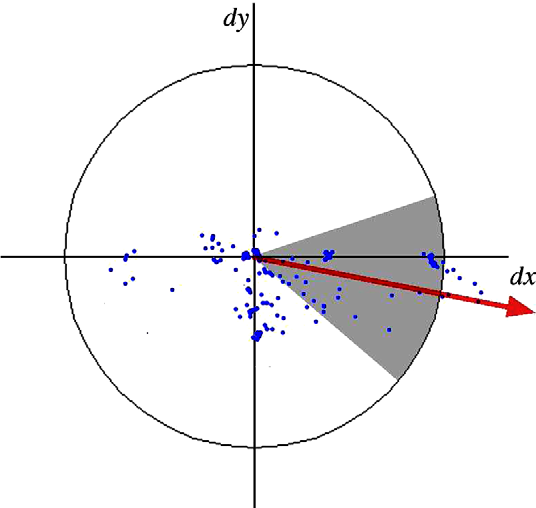
\includegraphics[height=5.5cm]{orientation_window}%
      \caption{sum $(d_x, d_y)$ over a window size $\frac{\pi}{3}$}%
      &
      \includegraphics[height=5.5cm]{feature_neighborhood}%
      \caption{windows defining neighborhood}%
    \end{tabularx}
  \end{figure}
\end{itemize}
\vfill


%%%%%%%%%%%%%%%%%%%%%%%%%%%%%%%%%%%%%%%%%%%%%%%%%%%%%%%%%%%%%%%%%%%%%%%%%%%%%%%%
\NewPage\headline{Image Features: Speeded Up Robust Features}
\vfill
\begin{itemize}
\item 4D descriptor vector $v = (\sum d_x, \sum d_y, \sum \lvert d_x \rvert, \sum \lvert d_y \rvert)$ for each sub-window $\Rightarrow$ 64D SURF descriptor.
\item Normalize to make it invariant to contrast (a scale factor).
%\item[]
\end{itemize}
  \begin{figure}
    \centering
    \begin{tabularx}{600pt}{Z Z}
      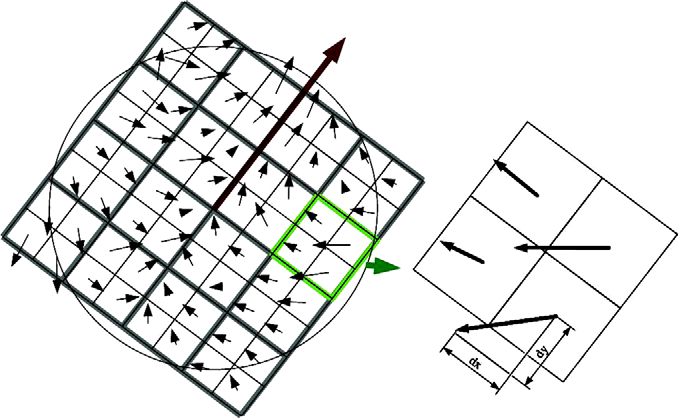
\includegraphics[width=0.4\textwidth]{surf}%
      \caption{Wavelet responses extracted from neighborhood}%
      &
      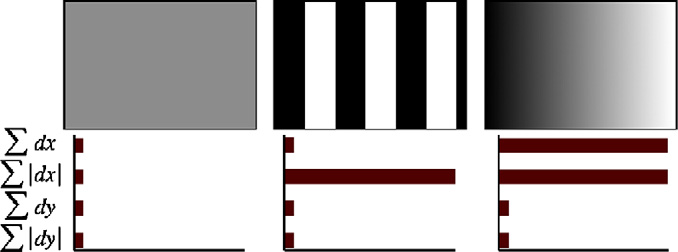
\includegraphics[width=0.4\textwidth]{surf_vector}%
      \caption{The descriptor entries represent the underlying intensity pattern.}%
    \end{tabularx}
  \end{figure}
\vfill


%%%%%%%%%%%%%%%%%%%%%%%%%%%%%%%%%%%%%%%%%%%%%%%%%%%%%%%%%%%%%%%%%%%%%%%%%%%%%%%%
\NewPage\headline{Gradient-based Features}
\small
\vfill
\begin{itemize}
\item Draw a circle with radius $r$, divide it along the diameter at orientation $\theta$.
\item Build histograms of brightness, color and texture for each disc half.
\item Compares histograms of the two disc halves: $G(x, y, \theta, r) = \chi ^ 2 (g, h) = \frac{1}{2} \sum_i \frac{(g_i - h_i)^2}{(g_i + h_i)}$
\item Use logistic regression trained on human segmentation dataset to get the result $Pb_{\sigma}(x, y, \theta)$.
\end{itemize}
\begin{figure}
	\centering
	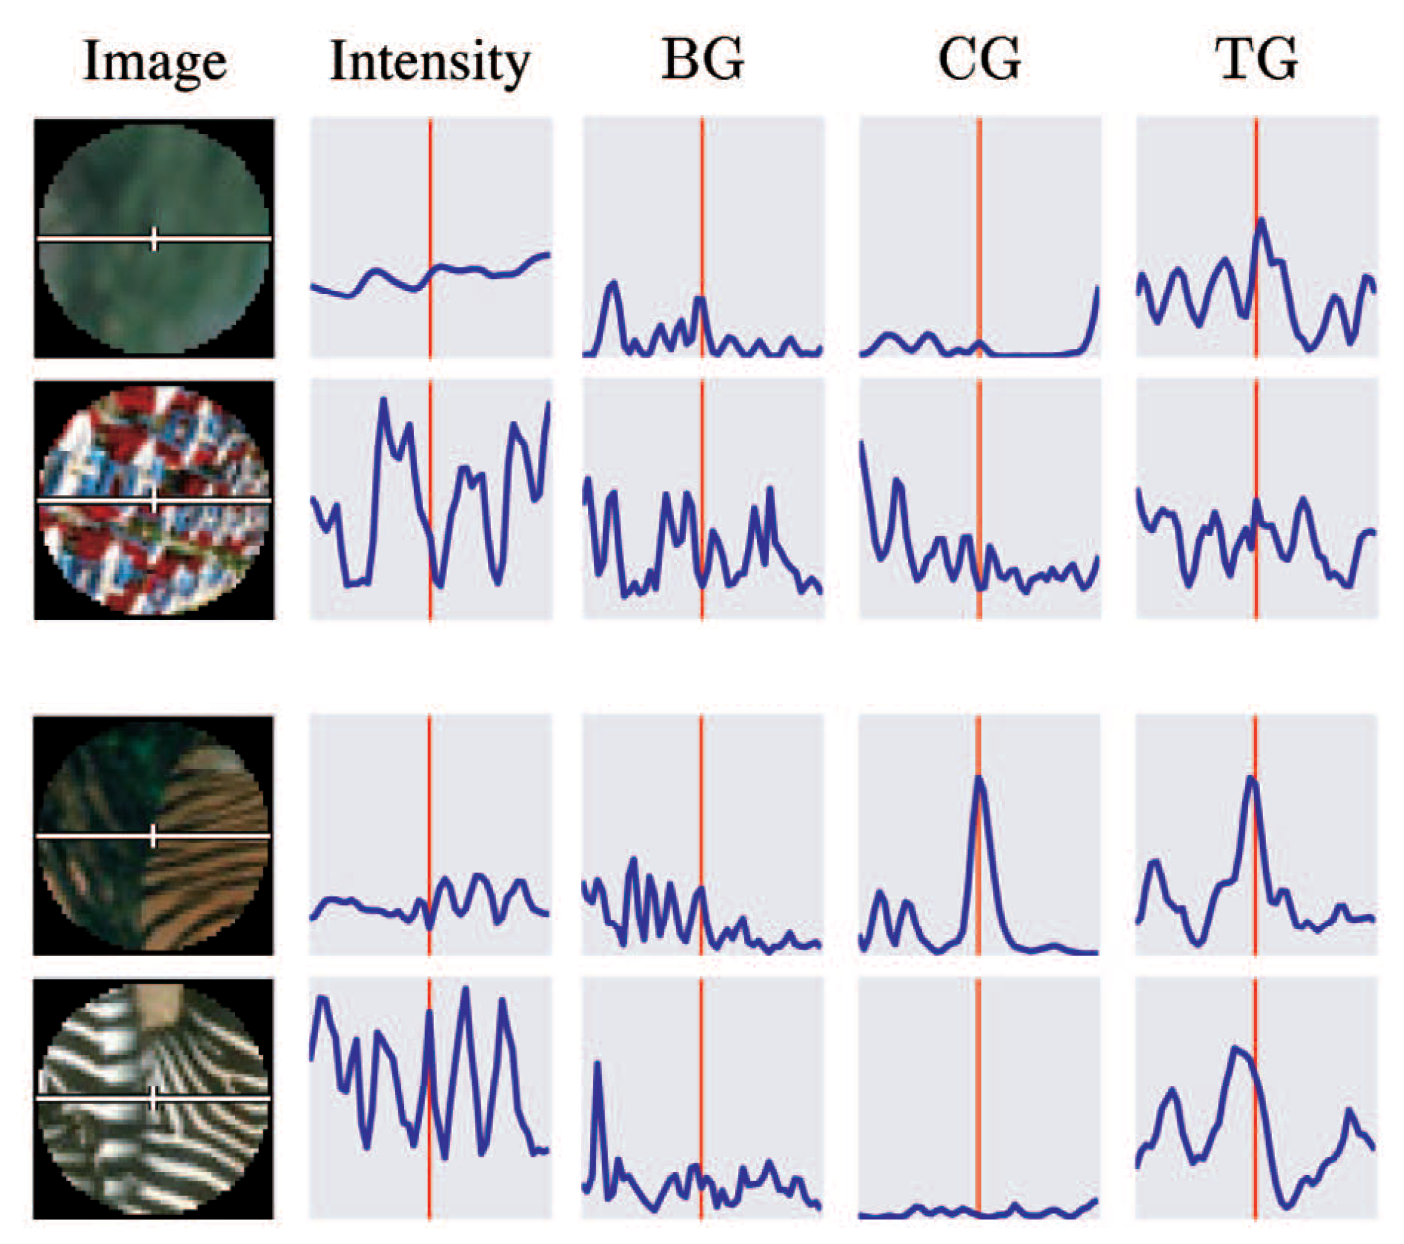
\includegraphics[width=0.45\textwidth]{gradient_features}
\end{figure}
\vfill


%%%%%%%%%%%%%%%%%%%%%%%%%%%%%%%%%%%%%%%%%%%%%%%%%%%%%%%%%%%%%%%%%%%%%%%%%%%%%%%%
\NewPage\headline{Globalized Probability of Boundary}
\small
\vfill
\begin{itemize}
\item Brightness, color and texture gradients in 3 different scales: $mPb(x, y, \theta) = \sum\limits_{i = 1}^{9} G_i(x, y, \theta)$.
\item Define affinity matrix $W$ using intervening contour cue $mPb$. Solve the generalized eigenvectors problem: $(D - W)v = \lambda D v$, $D_{ii} = \sum_j W_{ij}$.
\item Edges from generalized eigenvectors $v_j$: $sPb(x, y, \theta) = \sum\limits_{j = 1}^{k} \frac{1}{\sqrt{\lambda_j}} sPb_{v_j} (x, y, \theta)$.
\item Globalized probability of boundary: $gPb(x, y, \theta) = \sum\limits_{i = 1}^{9} \beta_iG_i(x, y, \theta) + \gamma sPb(x, y, \theta)$.
\end{itemize}
%  \begin{figure}
%    \centering
%    \begin{tabularx}{600pt}{Z Z}
%      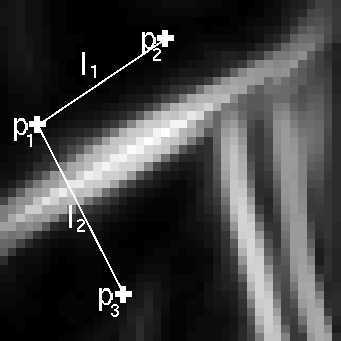
\includegraphics[width=0.15\textwidth]{intervening_contour2}%
%      \caption{Intervening contour}%
%      &
%      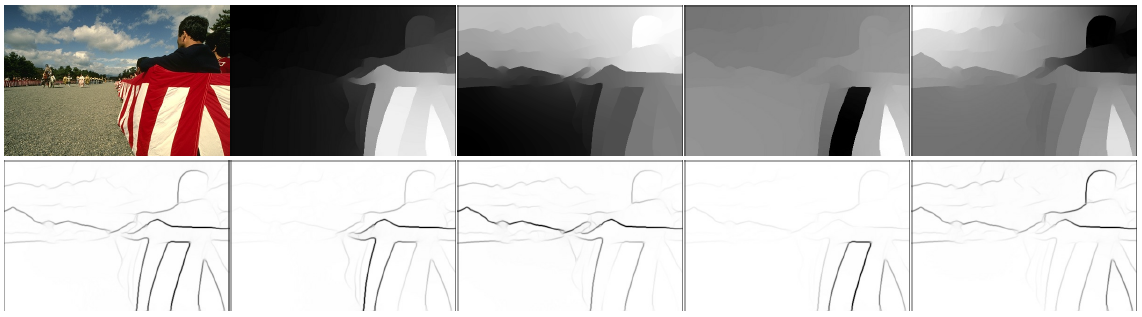
\includegraphics[width=0.55\textwidth]{sPb}%
%      \caption{Eigenvectors and their edges}%
%    \end{tabularx}
%  \end{figure}
\begin{table}
  \centering
  \begin{tabular}{@{} M{.3\linewidth} M{.7\linewidth} @{}}
      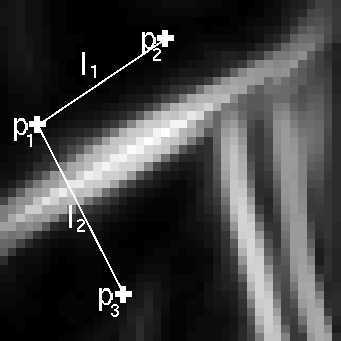
\includegraphics[width=0.15\textwidth]{intervening_contour2}%
      \caption{Intervening contour}%
      &
      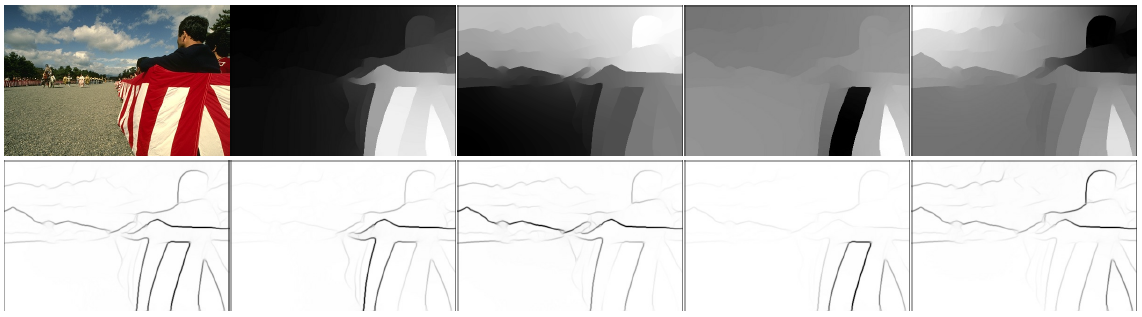
\includegraphics[width=0.65\textwidth]{sPb}%
      \caption{Eigenvectors and their edges}%
  \end{tabular}
\end{table}
\vfill





%%%%%%%%%%%%%%%%%%%%%%%%%%%%%%%%%%%%%%%%%%%%%%%%%%%%%%%%%%%%%%%%%%%%%%%%%%%%%%%%
\NewPage\headline{Including Images}
\vfill
\begin{itemize}
\item free positioning of images or texts using textboxes, look at the z-index
\end{itemize}
\vfill
\begin{textblock}{4}(2,-1) % in runden Klammern die Koordinaten, von der jeweiligen Textstelle aus berechnet
  \scalebox{0.8}{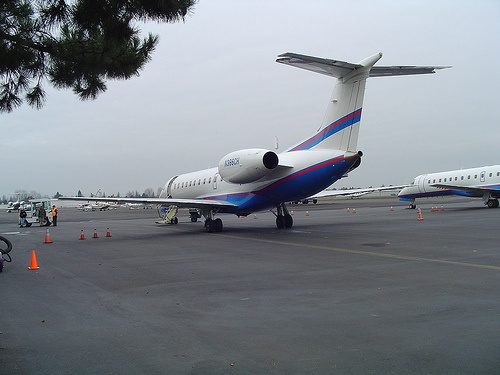
\includegraphics{airplane}}
\end{textblock} 
\begin{itemize}
\item \red{free positioning of images or texts using textboxes}
\end{itemize}
\begin{textblock}{4}(15,-2) % in runden Klammern die Koordinaten, von der jeweiligen Textstelle aus berechnet
  \scalebox{0.8}{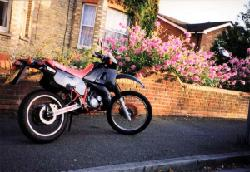
\includegraphics{motorbike}}
\end{textblock} 
\vfill






%%%%%%%%%%%%%%%%%%%%%%%%%%%%%%%%%%%%%%%%%%%%%%%%%%%%%%%%%%%%%%%%%%%%%%%%%%%%%%%%
\NewPage\headline{\LaTeX \ Tricks}
\vfill
Some \LaTeX\xspace tricks
\vfill




%%%%%%%%%%%%%%%%%%%%%%%%%%%%%%%%%%%%%%%%%%%%%%%%%%%%%%%%%%%%%%%%%%%%%%%%%%%%%%%%
\FinalPage
%%%

%%%


%%%%%%%%%%%%%%%%%%%%%%%%%%%%%%%%%%%%%%%%%%%%%%%%%%%%%%%%%%%%%%%%%%%%%%%%%%%%%%%%
\NewPage
%\headline{\refname}
%\renewcommand*{\refname}{}
\bibliographystyle{i6bibliostyle}
\bibliography{slides}

%\clearpage
\appendix
%%%%%%%%%%%%%%%%%%%%%%%%%%%%%%%%%%%%%%%%%%%%%%%%%%%%%%%%%%%%%%%%%%%%%%%%%%%%%%%%
\NewPage\headline{\appendixname: First Slide}
\vfill
\hypertarget{anchorname}{Hyper Target} on the first appendix slide. 
Look at the current page number.
\vfill

%%%%%%%%%%%%%%%%%%%%%%%%%%%%%%%%%%%%%%%%%%%%%%%%%%%%%%%%%%%%%%%%%%%%%%%%%%%%%%%%
\NewPage\headline{\appendixname: Table Data}
\vfill
\hypertarget{table_data}{Table Data} on the second appendix slide.
Look at the current page number.
\vfill

\end{document}
